\documentclass{article}
% Author: Luan Leal
% Last update: 2024-12-03

% ----------------------------

% ----------------------------   IMPORTS   ----------------------------
\usepackage{amssymb, amsthm, amsmath, geometry, siunitx, caption, float, graphicx}
\usepackage{enumitem}
\usepackage[utf8]{inputenc}
\usepackage[onehalfspacing]{setspaceenhanced}
\usepackage[brazil]{babel} % Adaptação ao pt-br
\usepackage{hyperref} % Usado para inserir links
\usepackage[capitalize, brazilian, noabbrev]{cleveref} % Referência adaptada ao pt-br
\usepackage{subcaption}
\usepackage{makecell}
\usepackage[num,overcite]{abntex2cite}

% ----------------------------   LAYOUT   ----------------------------
\citebrackets[]
\geometry{a4paper, lmargin=3cm, tmargin=3cm, rmargin=2cm, bmargin=2cm}
\onehalfspacing
%\setlength{\parindent}{45pt}
\sisetup{output-decimal-marker = {,}}

% ----------------------------  THEOREMS  ----------------------------
% -Ambiente de definição
\theoremstyle{definition}
\newtheorem{dfn}{Definição}[section]

% -Ambiente de observação
\theoremstyle{remark}
\newtheorem{obs}{Observação}

% -Ambiente de lema
\theoremstyle{definition}
\newtheorem{lema}{Lema}

% -Ambiente de exemplo
\theoremstyle{definition}
\newtheorem{xp}{Exemplo}[section]

% -Ambiente de proposição
\newtheorem{prop}{Proposição}

% -Ambiente de teorema e demonstração
\theoremstyle{plain}
\newtheorem{thm}{Teorema}
\theoremstyle{remark}
\newtheorem*{dms}{Demonstração}

% -Ambiente de exercício e resolução
\theoremstyle{definition}
\newtheorem{xcs}{Exercício}
\theoremstyle{remark}
\newtheorem*{rsl}{Resolução}

% ----------------------------  COMMANDS  ----------------------------
%\newcommand{\RR}{\mathbb{R}} % \mathbb{R} = \RR
%\newcommand{\ZZ}{\mathbb{Z}} % \mathbb{Z} = \ZZ

\author{Luan Leal (15470820);
; Matheus Queiroz (15479562);\\ Micael Baruch (15578823)}
\title{Relatório 3} 

\captionsetup{margin=10pt,font=small,labelfont=bf,labelsep=period}

\begin{document}
\maketitle

\textbf{Questão 1}
\begin{figure}[H]
    \centering
    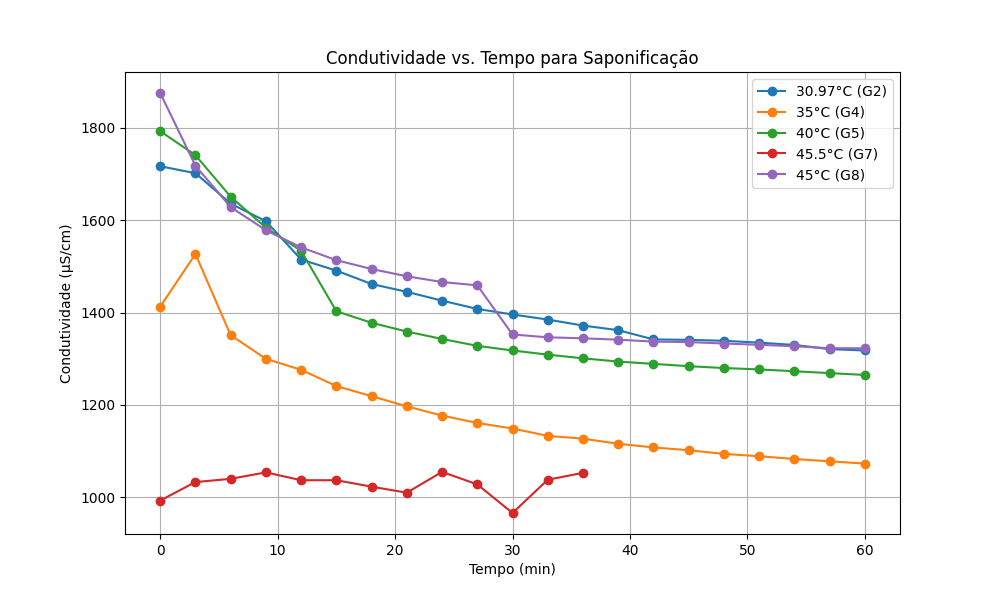
\includegraphics[width=.5\linewidth]{figs/graph1.png}
\end{figure}
\textbf{Questão 2}
\begin{figure}[H]
    \centering
    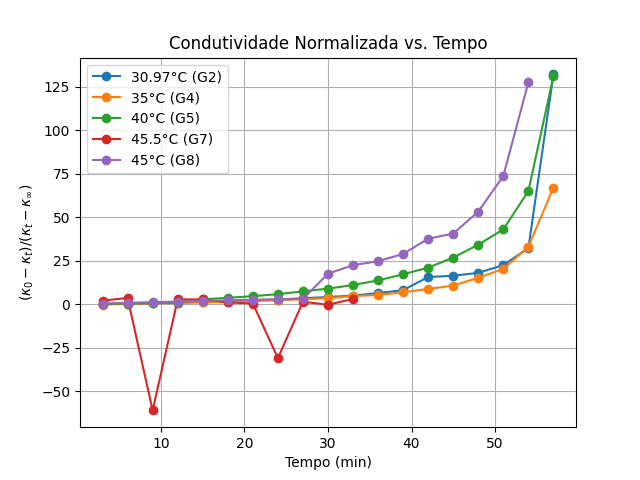
\includegraphics[width=.5\linewidth]{figs/graph2.png}
\end{figure}
\textbf{Questão 3}
\begin{figure}[H]
    \centering
    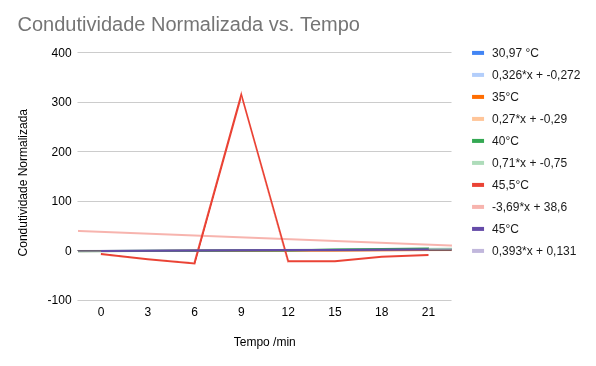
\includegraphics[width=.5\linewidth]{figs/graph3.png}
\end{figure}
\textbf{Questão 4}
\begin{table}[H]
\centering
\caption{Valores de $k$ normalizado em diferentes temperaturas e tempos.}
\label{tab:k_norm}
\begin{tabular}{lrrrrrrr}
\toprule
\textbf{Temperatura ($^{\circ}$C)} & \multicolumn{7}{c}{\textbf{Tempo (min)}} \\
\cmidrule(lr){2-8}
 & \multicolumn{1}{c}{3} & \multicolumn{1}{c}{6} & \multicolumn{1}{c}{9} & \multicolumn{1}{c}{12} & \multicolumn{1}{c}{15} & \multicolumn{1}{c}{18} & \multicolumn{1}{c}{21} \\
\midrule
30.97 (G2) & 1.32 & 4.31 & 4.79 & 8.67 & 8.84 & 9.99 & 10.35 \\
35 (G4)    & -8.50 & 3.77 & 5.62 & 5.71 & 6.93 & 7.49 & 8.42 \\
40 (G5)    & 3.70 & 6.22 & 7.39 & 8.15 & 19.13 & 20.71 & 22.32 \\
45 (G8)    & 13.51 & 13.69 & 13.13 & 12.95 & 12.85 & 12.53 & 12.32 \\
\bottomrule
\end{tabular}
\end{table}
\textbf{Questão 5}
\textbf{Questão 6}
\textbf{Questão 7}

    \bibliographystyle{plain}
    \bibliography{bibliography}

\end{document}
